\documentclass[border=10pt]{standalone}
\usepackage[svgnames]{xcolor}
\usepackage{amsmath}
\usepackage{pgfplots}
\pgfplotsset{compat=newest}
\usepackage[sfdefault]{FiraSans}
\usepackage{FiraMono}
\renewcommand*\familydefault{\sfdefault}
\begin{document}
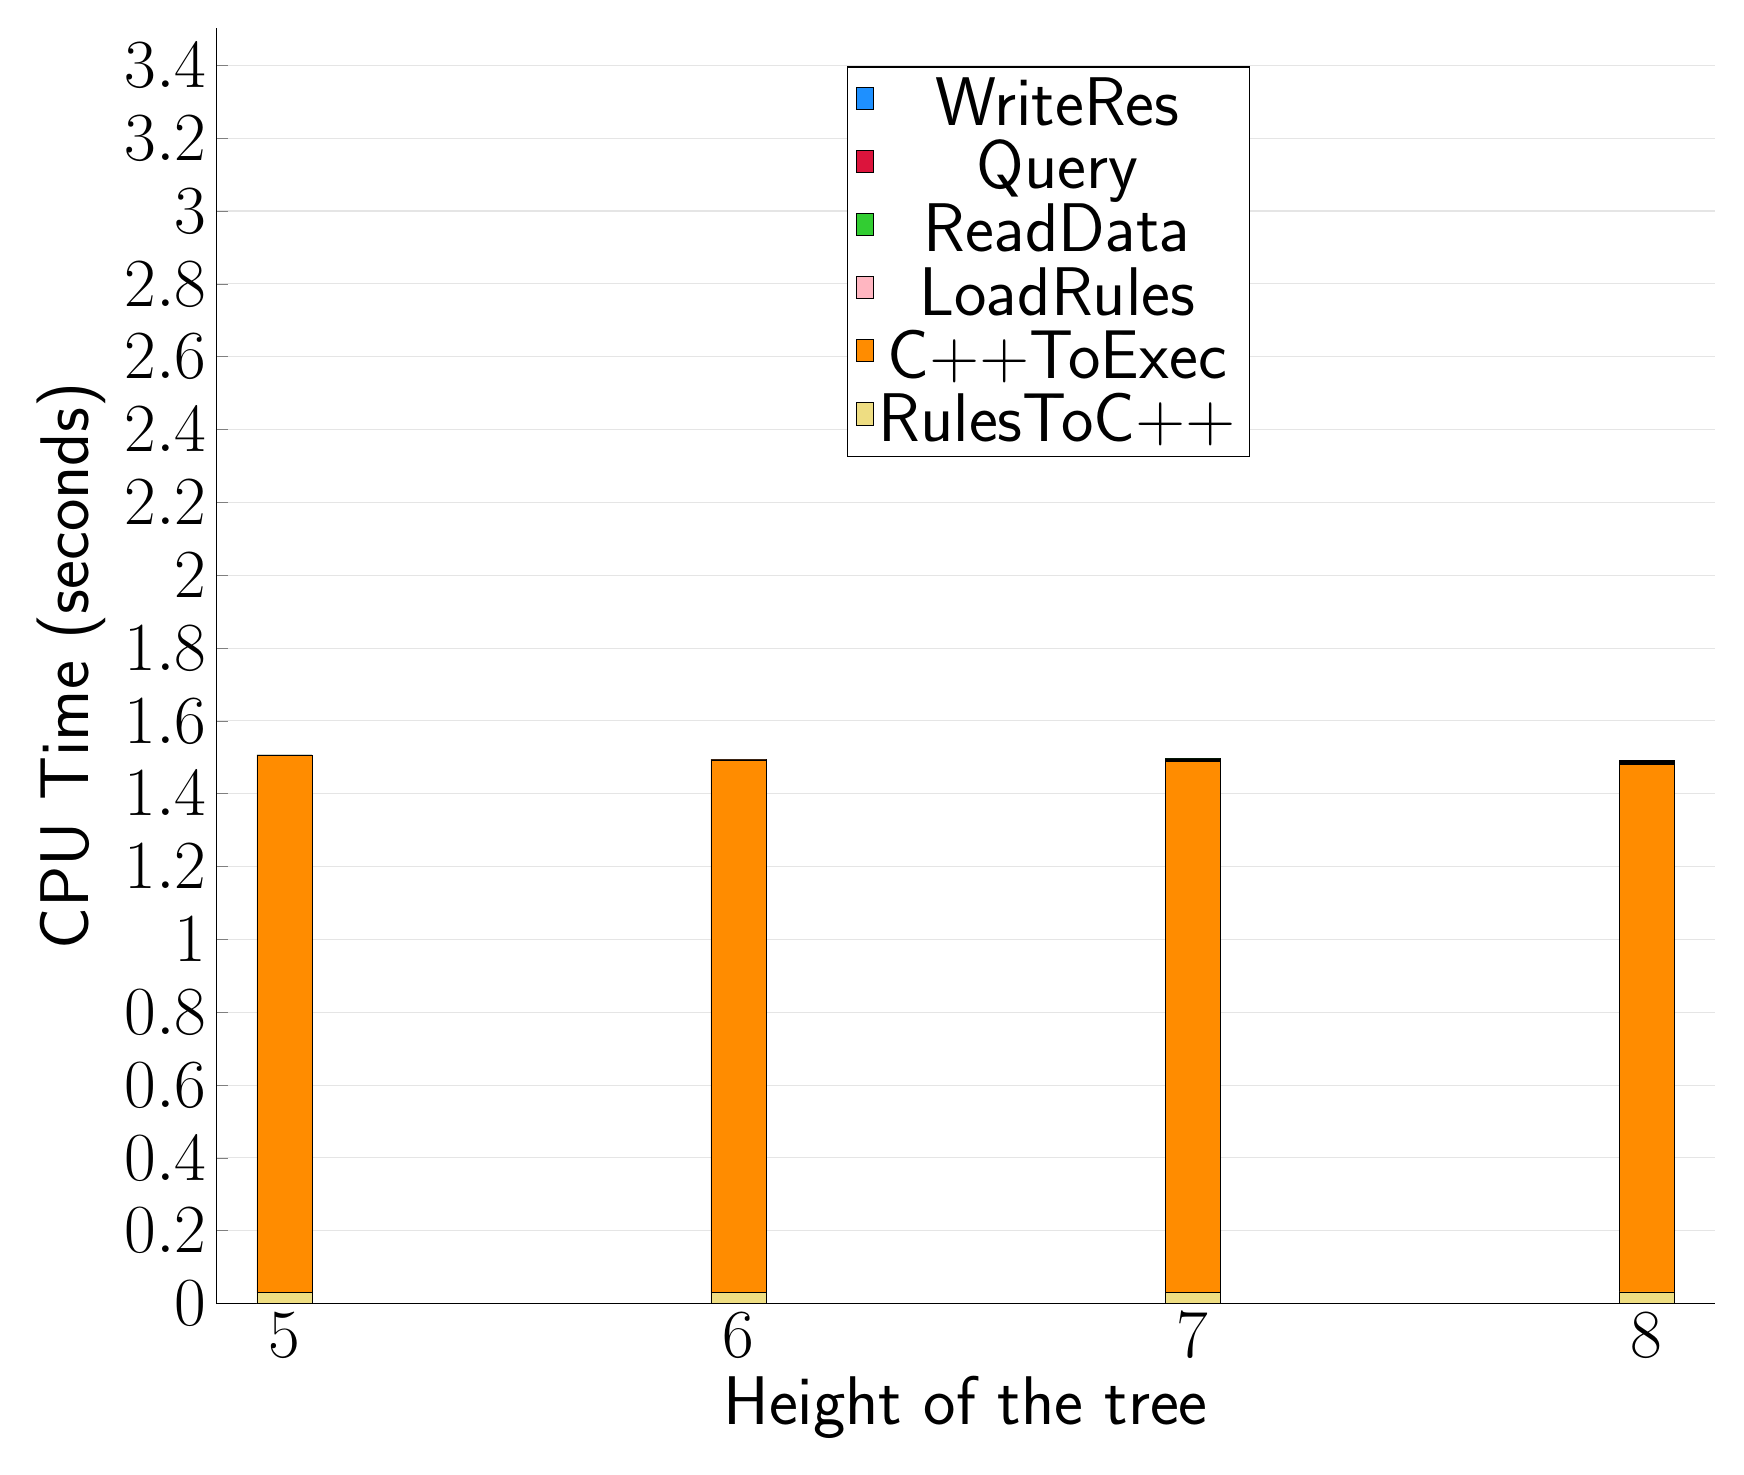
\begin{tikzpicture}
\begin{axis}[
   ybar stacked,
   width=1.7\textwidth,
   bar width=0.7cm,
   ymajorgrids, tick align=inside,
   major grid style={draw=gray!20},
   xtick=data,
   ymin=0, ymax=3.5020000000000002,
   axis x line*=bottom,
   axis y line*=left,
   enlarge x limits=0.05,
   legend style={
       at={(0.69, 0.97)},
       anchor=north east,
       legend columns=1,
       font=\Huge,
   },
   ylabel={CPU Time (seconds)},
   xlabel={Height of the tree},
   label style={font=\Huge},
   tick label style={font=\Huge},
]
\addlegendimage{fill=DodgerBlue, draw=black, line width=0.2pt}
\addlegendentry{WriteRes}
\addlegendimage{fill=Crimson, draw=black, line width=0.2pt}
\addlegendentry{Query}
\addlegendimage{fill=LimeGreen, draw=black, line width=0.2pt}
\addlegendentry{ReadData}
\addlegendimage{fill=LightPink, draw=black, line width=0.2pt}
\addlegendentry{LoadRules}
\addlegendimage{fill=DarkOrange, draw=black, line width=0.2pt}
\addlegendentry{C++ToExec}
\addlegendimage{fill=LightGoldenrod, draw=black, line width=0.2pt}
\addlegendentry{RulesToC++}
\addplot +[fill=LightGoldenrod, draw=black, line width=0.2pt] coordinates {
(5, 0.030000000000000006)
(6, 0.030000000000000006)
(7, 0.030000000000000006)
(7, 0.030999999999999993)
(7, 0.030000000000000006)
(8, 0.030000000000000006)
(8, 0.030000000000000006)
(8, 0.032)
};
\addplot +[fill=DarkOrange, draw=black, line width=0.2pt] coordinates {
(5, 1.4759999999999998)
(6, 1.4629999999999999)
(7, 1.4609999999999996)
(7, 1.457)
(7, 1.465)
(8, 1.457)
(8, 1.454)
(8, 1.4479999999999997)
};
\addplot +[fill=LightPink, draw=black, line width=0.2pt] coordinates {
(5, 0.00012389999999999998)
(6, 0.0001121)
(7, 0.00012429999999999999)
(7, 0.0001245)
(7, 0.0001229)
(8, 0.0001245)
(8, 0.0001229)
(8, 0.0001226)
};
\addplot +[fill=LimeGreen, draw=black, line width=0.2pt] coordinates {
(5, 0.0003083)
(6, 0.0003834)
(7, 0.0005181)
(7, 0.0005258000000000001)
(7, 0.0005255)
(8, 0.0008077000000000001)
(8, 0.0007971)
(8, 0.0008090999999999999)
};
\addplot +[fill=Crimson, draw=black, line width=0.2pt] coordinates {
(5, 0.0001448)
(6, 0.0003242)
(7, 0.0007469)
(7, 0.0007865000000000001)
(7, 0.0007790999999999998)
(8, 0.0018917)
(8, 0.0018633)
(8, 0.0018651000000000002)
};
\addplot +[fill=DodgerBlue, draw=black, line width=0.2pt] coordinates {
(5, 0.0002637)
(6, 0.0003499)
(7, 0.0005118)
(7, 0.0005184)
(7, 0.0005001999999999999)
(8, 0.0009649)
(8, 0.0009237000000000001)
(8, 0.00092)
};
\end{axis}
\end{tikzpicture}

\end{document}
